%!TEX root = ../main.tex



\noindent
This chapter is mainly based on a paper from Karl Wüst and Arthur Gervais titled \href{https://eprint.iacr.org/2017/375.pdf}{Do you need a blockchain}.
The Figure 1 below is taken from the same paper.

\begin{figure}[h!]
	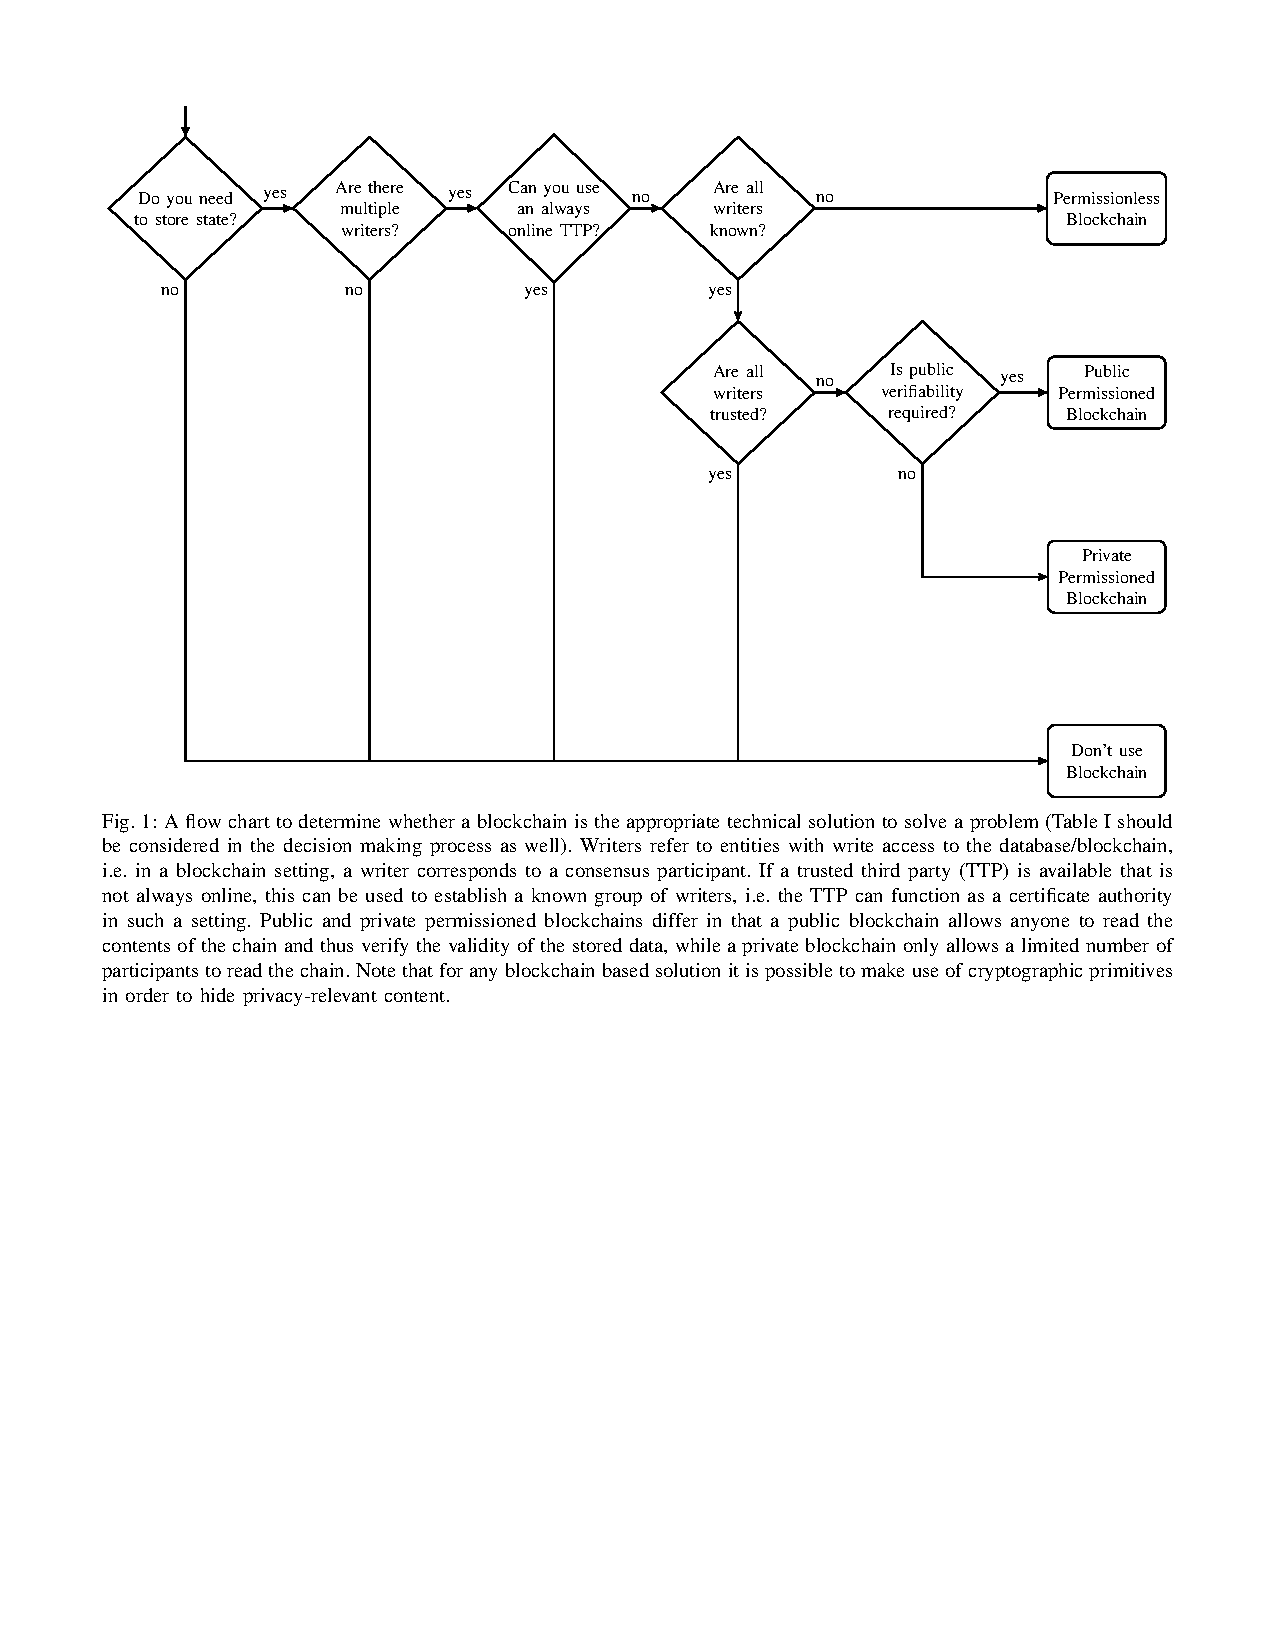
\includegraphics[width=\textwidth]{fig/FlowChart}
	
\end{figure}

\section{Supply chain}
Managing inventory, orders, processes, and failures in supply chains is a complex and expensive process. 
Improved data sharing between different parties has a big potential to improve supply chains.
A blockchain may additionally improve traceability and prevent fraud.


\begin{itemize}
	\item[] \textbf{Limitations:}
	\begin{itemize}	
	\item Data sharing is possible without a blockchain.
	\item Traceability is limited, due to the oracle problem, i.e., logged events on blockchain may not coincide with real world.
	\item Scalability might be an issue.
	\end{itemize}
	\item[] \textbf{Opportunities:}
	It seems especially for items that require thorough documentation, e.g., ivory or diamonds blockchain might be useful.
\end{itemize}

\section{Inter bank payments}
Today national inter bank payments are managed via national central banks.
International inter bank payments are managed by multiple national banks.
The system is expensive and complex.

A blockchain based approach may be a promising solution.

\begin{itemize}
	\item[] \textbf{Limitations:}
	Success depends on regulators. If appeals can be made by an external court, the system may become incorrect.
\end{itemize}

\section{Digital services}
When providing digital services, blockchains may have a good standing. Potential services are: Data storage, data exchange, dns resolution, search and lookup.

\begin{itemize}
	\item Can systems be as trustful as centralized systems?
	\item Can systems improve privacy compared to centralized systems?
\end{itemize}

